
\documentclass[smallextended]{svjour3}[2017 April 7th]

\usepackage{amssymb}
\usepackage{amsmath,dsfont}
\usepackage[ruled,vlined, linesnumbered]{algorithm2e}
\usepackage{pgfplots}
\usepackage[utf8]{inputenc}
\usepackage{url}
\usepackage{tikz}
\usepackage{caption}
\usepackage{subfig}
\tikzset{
  font={\fontsize{9pt}{12}\selectfont}}
\newtheorem{oss}{Remark}

\newcommand{\R}{\mathbb{R}}
\newcommand{\N}{\mathbb{N}}
\DeclareMathOperator*{\argmin}{arg\,min}
\definecolor{gr}{HTML}{00BB00}
\setlength\parindent{0pt}


\begin{document}


%% Title, authors and addresses

%% use the tnoteref command within \title for footnotes;
%% use the tnotetext command for theassociated footnote;
%% use the fnref command within \author or \address for footnotes;
%% use the fntext command for theassociated footnote;
%% use the corref command within \author for corresponding author footnotes;
%% use the cortext command for theassociated footnote;
%% use the ead command for the email address,
%% and the form \ead[url] for the home page:
%% \title{Title\tnoteref{label1}}
%% \tnotetext[label1]{}
%% \author{Name\corref{cor1}\fnref{label2}}
%% \ead{email address}
%% \ead[url]{home page}
%% \fntext[label2]{}
%% \cortext[cor1]{}
%% \address{Address\fnref{label3}}
%% \fntext[label3]{}

\title{Globally convergent decomposition algorithm for risk parity problem in portfolio selection}

%% use optional labels to link authors explicitly to addresses:
%% \author[label1,label2]{}
%% \address[label1]{}
%% \address[label2]{}

\author{A.Cassioli\and G.Cocchi \and F.D'Amato\and M.Sciandrone}

\institute{A.Cassioli \at MOSEK ApS, Copenhagen, Denmark, \email{andrea.cassioli@mosek.com}}
\institute{G.Cocchi \and F.-D'Amato \and M.Sciandrone \at Dipartimento di Ingegneria dell'Informazione, Università di Firenze, Firenze, Italy, \email{guido.cocchi@unifi.it},\email{federico.damato@stud.unifi.it},\email{marco.sciandrone@unifi.it}
}

\begin{abstract}
The abstract

\end{abstract}
%% \linenumbers

%% main text
\section{Introduction}
%%write something
The most important problem in budget allocation is making a good porfolio in terms of expected return and volatility. 
A lot of models were based on the Markowitz theory, stated in 1950s, for finding portfolio in the efficient frontier. 
All these approaches are proved to be unsuitable to real contexts, due to the market unstability and the ill-conditions of the problems. 
% aggiungere diversificazione
So the scientific community did a lot of works to find a way to minimize only the risk or the diversification. 
Many naive techniques as Equally Weighting (EW) portfolios were adopted in several real contexts showing poor perfomance, altought they have good theoretical performance. 
The Risk Parity concept was proposed in \cite{qian2005} to construct a portfolio such that all the asset contributions to the total risk are equal to each other \cite{maillard}.
Many different formulations were used to deal with Risk Parity, depending also on the absence of the \emph{short-selling} constraint (i.e. $x\ge0$).
In \cite{maillard} a nonlinear nonconvex least-squares optimization model without short-selling constraint was proposed.

In \cite{tardella2016} an equally bounded risk formulation was proposed, in which all the risk contributions are equally upper bounded by the same variable. It can be proved that an optimal solution for the long-short ERB is also a Risk Parity solution with minimum variance.
In \cite{feng2016} a scalarized version of a multi-objective optimization problem considering the expected return the risk the sparsity and the risk parity was addressed with a successive convex approximations.
In \cite{tutuncu} a lightly modification of the least-squares approach was proposed considering another optimization variable $\theta$ which represents the value around which all risk contribution will stay.
\begin{subequations}\label{eq:problemRP} 
\begin{align}
\min_{x,\theta} & \quad f(x,\theta) =  \sum_{i=i}^n \left(x_i(Q x)_i - \theta\right)^2 \\
\text{s.t.} & \quad l \leq x \leq u \\
& \quad \mathds{1}^T x = 1 
\end{align}
\end{subequations}
Due to its more readable form and its lower evaluating cost, we consider that formulation as our optimization problem.
Because of Sequential Quadratic Programming has poor performance when the number of assets increases, we proposed a globally convergent decomposition algorithm which uses a two level decomposition framework.
We use a Gauss-Seidel decomposition with respect to the two blocks $x,\theta$, then when we have to optimize the $x$ block we use a Gauss-Southwell decomposition which select the Most Violating Pair for the optimality conditions among all the asset variables. Then we decrease the objective function with a line search considering only the MVP pair.

The paper proceeds as follow: in section blablablabla.


\begin{proposition}
evbrfretre
\end{proposition}
\clearpage
\section{Preliminary background}\label{sect:2}
Let us consider the following optimization problem:
\begin{subequations}\label{eq:problem} 
\begin{align}
\min_{x,y} & \quad f(x,y)  \\
\text{s.t.} & \quad l \leq x \leq u \\
& \quad \mathds{1}^T x = 1 
\end{align}
\end{subequations}
where $x \in \R^n$, $y \in \R^m$, $f$ continuously differentiable, $l, u \in \R^n$ with $l < u$ and $\mathds{1} \in \R^n$ is all composed by ones. 

We define the feasible set $\mathcal{F}$  of Problem (\ref{eq:problem}):
\begin{equation}
\mathcal{F} = \{(x,y) \in \R^{n+m} : \mathds{1}^T x = 1, l \leq x \leq u\}.
\end{equation}
A vector $d\in \R^{n+m}$ is partitioned as follows
$$
d=\left(
\begin{array}{c}
d_x\\
d_y
\end{array}
\right ),
$$
where $d_x\in R^n$ and $d_y\in R^m$.

Given $(x,y) \in \mathcal{F}$, the set of feasible directions in $(x,y)$ is the cone
\begin{equation}
 \mathcal{D}(x,y)=\{ d \in \R^{n+m}: \mathds{1}^Td_x=0, d_i\ge 0 \ \forall i \in L(x), d_i\le 0 \ \forall i \in U(x)\}
\end{equation}
where
\begin{equation}
 \begin{aligned}
  &L(x)=\{ i: \ x_i=l_i\}\\
  &U(x)=\{ i: \ x_i=u_i\}
 \end{aligned}
\end{equation}
Given $(\bar x,\bar y) \in \mathcal{F}$, we say that $(\bar x,\bar y)$ is a {\it critical point} if
$$
\nabla f(\bar x,\bar y)^Td\ge 0\quad\quad \forall d\in  \mathcal{D}(\bar x,\bar y).
$$
We can state the following result.

\begin{proposition}[Name]
\label{optimality}
A point $(\bar x,\bar y) \in \mathcal{F}$ is a critical point if and only if
\begin{equation}\label{on_x}
\begin{aligned}
&\nabla_xf(\bar x,\bar y)^Td_x\ge 0 \quad \forall d_x\in R^n & \\ 
&\text{s.t.} \quad \mathds{1}^Td_x=0,\quad d_i\ge 0 \ \forall i \in L(\bar x), \quad d_i\le 0 \ \forall i \in U(\bar x)&
\end{aligned}
\end{equation}
\begin{equation}\label{on_y}
 \nabla_yf(\bar x,\bar y)=0.
\end{equation} 
\end{proposition}


In correspondence to a feasible point $(x,y)$ we introduce the index sets
$$
R(x)=L(x)\cup C(x)
$$
$$
S(x)=U(x)\cup C(x),
$$
where 
$$
C(x)=\{i: l_i<x_i<u_i\}.
$$
We can state the following propositions (Propositions 2.2 and 2.3 in Jota2009).
\begin{proposition}\label{2.2}
 A feasible point $(\bar x,\bar y)$ is a critical point if and only if for each pair $(i,j)$,
$i\in R(\bar x)$, $j\in S(\bar x)$, we have
\begin{equation}\label{on_RS}
 {{\partial f(\bar x,\bar y)}\over{\partial x_i}}\ge
 {{\partial f(\bar x,\bar y)}\over{\partial x_j}}
\end{equation}
\begin{equation}\label{on_y2}
\nabla_yf(\bar x,\bar y)=0.
\end{equation}
\end{proposition}
\begin{proposition}\label{2.3}
 Let $\{(x^k,y^k)\}$ be a sequence of feasible points convergent to a point $(\bar x,\bar y)$.
Then, for sufficiently large values of $k$, we have
$$
R(\bar x)\subseteq R(x^k) \quad \quad {\rm and}\quad \quad S(\bar x)\subseteq S(x^k).
$$
\end{proposition}

\subsection{Set of sparse feasible directions}
In our decomposition framework we will employ feasible directions having only two
nonzero components.
Then, in this subsection we introduce these sparse feasible directions and we show their important properties.

Given $i, j\in  \{1, \ldots ,n\}$, with $i\ne j$,
we indicate by $d^{i,j}\in  \R^{n+m}$ such that
\begin{equation}\label{eq:direction}
d_h^{i,j}= 
\begin{cases}
1, \quad \text{    } h=i\\
-1, \text{    } \text{    } h=j\\
0, \quad \text{    } \text{otherwise}
\end{cases}
\end{equation}
Note that, by definition, the components $d_h^{i,j}$ with $h=n+1,\ldots,n+m$ are always set to zero.

Given $(x, y) \in \mathcal{F}$ and the corresponding index sets $R(x)$ and $S(x)$, we indicate by $D_{RS}(x,y)$
the set of directions $d^{i,j}$ with $i \in R(x)$ and $j \in S(x)$, namely
$$
D_{RS}(x,y)=\cup_{i\in R(x),j\in S(x)}d^{i,j}.
$$
\begin{proposition}\label{3.1}
Let $(\bar x,\bar y)$ be a feasible point. For each pair $i \in R(x)$ and $j \in S(x)$, the
direction $d^{i,j}\in \R^{n+m}$ is a feasible direction at $(\bar x,\bar y)$, i.e. $d \in D(\bar x,\bar y)$.
\end{proposition}
\begin{proposition}\label{3.2}
A feasible point $(\bar x,\bar y)$
 is a critical point if and only
\begin{equation}\label{on_x2}
\nabla f(\bar x,\bar y)^Td^{i,j}\ge 0\quad\quad \forall d^{i,j}\in D_{RS}(\bar x,\bar y)
\end{equation}
\begin{equation}\label{on_y3}
 \nabla_y f(\bar x,\bar y)=0.
\end{equation} 
\end{proposition}
Given a feasible point $(\bar x,\bar y)$, a pair $i\in R(\bar x)$ and $j\in S(\bar x)$ such that
$$
\nabla f(\bar x,\bar y)^Td^{i,j}<0
$$
is said a {\it Violating Pair} (VP).

A violating pair $(i^\star,j^\star)$ such that 
\begin{equation}\label{mvp}
 \nabla f(\bar x,\bar y)^Td^{i^\star,j^\star}\le \nabla f(\bar x,\bar y)^Td^{i,j} \quad \forall i\in R(\bar x), \ j\in S(\bar x).
\end{equation}
is the {\it Most Violating Pair} (MVP).



\clearpage
\section{A general decomposition framework}
As already discussed, we partition the vector of variables into two blocks in order to take into account
the structure of the feasible set and possibly the form of the objective function (see, for instance,
the formulation of the risk parity problem, where the objective function is convex w.r.t. the scalar variable $\theta$).
The first block contains the constrained variables $x$, the second block contains
the unconstrained variables $y$. 

A first possibility can be that of defining a two-blocks Gauss-Seidel algorithm.
According to this scheme, at each iteration, the two component vectors $x$ and $y$ are
sequentially updated by performing  minimization steps (either exact or inexact) by  suitable descent techniques.
Globally convergent results of Gauss-Seidel algorithms (both exact and inexact) have been established in \cite{}, \cite{}, \cite{}.

We present here a block descent algorithm where a further level of decomposition is
introduced with respect to the block component $x$. 
More specifically, at each iteration, only two variables are updated, those corresponding
to a {\it Violating Pair}, by performing an inexact line search along a feasible and descent direction.
In order to guarantee convergence, the {\it Most Violating Pair} must be selected at least periodically, say every $M$ iterations.
We will discuss in the section of the computational experiments the role and the influence of the parameter $M$.

The adoption of a decomposition strategy with respect to the subvector $x$ is suitable
whenever the number $n$ of variables is large.

Note that the properties of the standard Armijo-type line search do not guarantee, without further assumptions
on the descent search direction $d^k$, that the distance between successive points tends to zero, which is a usual requirement of decomposition methods. 
This motivates the employment of the Quadratic Line Searck (QLS) defined in the appendix and based on the acceptance condition
$$
f((x^k,y^k)+\alpha^kd^k)\le f((x^k),y^k))-\gamma (\alpha^k)^2\|d^k\|^2.
$$
Concerning the unconstrained block component $y$, we do not specify the updating rule, but we state the following assumption that
could be satisfied, in practice, by different techniques depending on the hypothesis on $f$.
\par\medskip\noindent
{\bf Assumption on the updating rule of} $y$.
\par\medskip\noindent
\begin{itemize}
\item[(i)] For each $k$ we have $f(x^k,y^{k+1})\le f(x^k,y^k)$
\item [(ii)] If
$$
\lim_{k\to\infty} \left(f(x^k,y^{k+1})- f(x^k,y^k)\right)=0
$$
then
$$
\lim_{k\to\infty}\|y^{k+1}-y^k\|=0
$$
and
$$
\lim_{k\to\infty}\nabla_y f(x^k,y^k)=0.
$$
\end{itemize}


%At every step $k$ we choose a random subset $W^k\subset \{1,..,n\}$ such as
%\begin{equation}\label{eq:lambda}
%\frac{|W^k|}{n} \times 100 = \lambda
%\end{equation}
%For each $w \in W^k$, we compute the partial derivative $\frac{\partial f(x,\theta)}{\partial x_w}$ and 
%we select the MVP among the indexes in $W^k$. If we don't find a violating pair in $W^k$, 
%we randomly add indexes until we find one, and we use this violating pair to build the descent direction. To assure the global convergence properties, we evaluate the MVP among the full gradient $\nabla_x f(x,\theta)$ every $M$ iterations. \\
The algorithm is formally described below.

\begin{algorithm}[ht]
 \KwData{Given the initial feasible point $(x^{0}, y^{0})$}
 Set $k = 0$\\
 \While{(not convergence)}{
  Compute $y^{k+1}$ such that Assumptions (i) and (ii) hold\\
 \eIf{$k \enskip \text{mod} \enskip M = 0$}
  {
  Let $(i(k), j(k))$ be a Most Violating Pair\\ 
  }
  {
  Let $(i(k), j(k))$ be a Violating Pair\ 
  }
  Compute a step $\alpha^{k}$  along the direction $d^k=d^{i(k),j(k)}$ by QLS\\
  Set $x_{i(k)}^{k+1} = x_{i(k)}^{k} + \alpha^{k}$, $x_{j(k)}^{k+1} = x_{j(k)}^{k} - \alpha^{k}$  \\

  Set $k = k + 1$
 }
 \caption{Decomposition Algorithm}
\end{algorithm}
\par\bigskip\noindent
We can prove the following global convergence result.
\begin{proposition}\label{prop:conv1}
Suppose that the level set $\mathcal{L}_0$ is a compact set. Let $\{(x^k, y^k)\}$ be the sequence of points generated by the decomposition algorithm. Then
$\{(x^k, y^k)\}$ admits limit points and each limit point is critical for Problem (\ref{eq:problem}).
%\end{itemize}
\end{proposition}

\begin{proof}
The instructions of the algorithm imply
$$
f(x^{k+1}, y^{k+1})\le f(x^{k}, y^{k+1}) \leq f(x^{k}, y^{k}),
$$
so that, the points of the sequence $\{(x^{k}, y^{k})\}$ belongs to the compact set $\mathcal{L}_0$.
We also have
\begin{equation}\label{on_funct}
 \lim_{k\to\infty} f(x^k,y^{k+1})=\lim_{k\to\infty} f(x^{k},y^{k})=\bar f>-\infty
\end{equation}
Let $(\overline{x},\overline{y})$ be a limit point of $\{(x^k, y^k)\}$, i.e. there exists an infinite subset $K \subseteq N$ such that
\begin{equation}\label{eq:asim}
\lim_{k \in K, k \rightarrow \infty} (x^k, y^k) = (\overline{x},\overline{y})
\end{equation}
By contradiction, let us assume that $(\overline{x},\overline{y})$ is not a critical point. 
In this case, at least one of the following conditions holds:
\begin{subequations}
\begin{align}
&\nabla_y f(\overline{x},\overline{y}) \neq 0  \label{eq:a}\\
&\exists \enskip i, j \enskip  \text{s.t.} \enskip d^{i,j}\in D(\bar x) \enskip  \text{and} \enskip  \nabla_x f(\overline{x},\overline{y})^T d^{i,j} = -\eta < 0 \label{eq:b}
\end{align}
\end{subequations}
Suppose that (\ref{eq:a}) holds.
From (\ref{on_funct}), Assumption (ii) on the updating rule of $y^k$, and the continuity of the gradient we get
$$
\lim_{k\to\infty}\nabla_y f(x^k,y^k)=\nabla_y f(\overline{x},\overline{y})=0,
$$
and this contradicts (\ref{eq:a}).

Now assume that (\ref{eq:b}) holds.
For each $k$, a stepsize $\alpha^k>0$ is computed by QLS along the descent direction $d^{i(k),j(k)}$.
Then we can write
\begin{equation}\label{red_funct}
 f(x^{k+1},y^{k+1})\le f(x^k,y^{k+1})-\gamma (\alpha^k)^2\|d^{i(k),j(k)}\|^2=f(x^k,y^{k+1})-\gamma\|x^{k+1}-x^k\|^2,
\end{equation}
from which, recalling (\ref{on_funct}) and that $\|d^{i(k),j(k)}\|^2=2$, we obtain
\begin{equation}\label{dst_x}
 \lim_{k\to\infty}\|x^{k+1}-x^k\|=\lim_{k\to\infty}\alpha^k=0.
\end{equation} 
From (\ref{on_funct}) and Assumption (ii) on the updating rule of $y^k$ we also have
\begin{equation}\label{dst_y}
 \lim_{k\to\infty}\|y^{k+1}-y^k\|=0.
\end{equation}
For each $k\in K$, let $v(k)$ be the integer such that $k+v(k)$ is an iteration
where the Most Violating Pair is selected. Note that we have
$$
0\le v(k) \le M.
$$
From (\ref{dst_x}) and (\ref{dst_y}) we obtain
\begin{equation}\label{cnv_x}
 \lim_{k\in K,k\to\infty}x^{k+v(k)}=\bar x
\end{equation}
\begin{equation}\label{cnv_y}
 \lim_{k\in K,k\to\infty}y^{k+v(k)+1}=\bar y.
\end{equation}
We introduce the index set 
$$
K_1=\{h: \ h=k+v(k), \ k\in K\}.
$$
By definition, for all $k\in K_1$ the Most Violating Pair $(i(k),j(k))$ is selected. Furthermore, we have
\begin{equation}\label{cnv2_x}
 \lim_{k\in K_1,k\to\infty}x^{k}=\bar x
\end{equation}
\begin{equation}\label{cnv2_y}
 \lim_{k\in K_1,k\to\infty}y^{k+1}=\bar y.
\end{equation}
Since $i(k)$ and $j(k)$ belong to the finite set $\{1,\ldots ,n\}$, we can extract a further subset (that we relabel by $K_1$) such that
$$
i(k)=i^\star \quad\quad j(k)=j^\star\quad\quad \forall k\in K_1.
$$
Note that $d^{i,j}\in D(\bar x,\bar y)$, so that, recalling Proposition \ref{2.3}, we obtain for
$k\in K_1$ and $k$ sufficiently large
\begin{equation}\label{dij_dk}
 d^{i,j}\in D(x^k,y^k).
\end{equation}
For all $k\in K_1$, as $(i^\star,j^\star)$ is the Most Violating Pair, using (\ref{dij_dk}) we can write
\begin{equation}\label{mvp_ij}
 \nabla_xf(x^k,y^{k+1})^Td^{i^\star,j^\star}\le \nabla_xf(x^k,y^{k+1})^Td^{i,j}<0.
\end{equation}
Then, $d^{i^\star,j^\star}$ is a feasible and descent direction, and hence a stepsize $\alpha^k$ is computed along it by QLS.
Further, from (\ref{dst_y}) and (\ref{eq:b}) it follows
\begin{equation}\label{desc_mvp}
 \nabla_xf(\bar x,\bar y)^Td^{i^\star,j^\star}<0.
\end{equation}
Now let us distinguish two cases:
\par\medskip\noindent
Case (I). There exists an integer $\ell$  such that
\begin{equation}\label{caseI}
 \alpha^{k+\ell(k)}<\Delta^{k+\ell(k)}
\end{equation}
for all $k\in K_1$ and for some $\ell(k)\le \ell$.
\par\medskip\noindent 
Case (II). For all $k\in K_1$ and $m=0,\ldots ,2n$ we have
\begin{equation}\label{caseII}
 \alpha^{k+m}=\Delta^{k+m}.
\end{equation}
{\it Case} (I)
\par\medskip\noindent
Without loss of generality assume $\ell (k)=0$.
Otherwise we can reason on the subsequence $\{x^k\}_{k+l(k)}$ that, by definition,
is a subsequence where the  MVP is selected again (see the new instruction) since $\alpha^{k+l(k)-s}=\Delta^{k+l(k)-s}$,
for $s=0,1,\ldots ,l(k)$,
and $\alpha^{k+l(k)}<\Delta^{k+l(k)})$.

The instructions of QLS imply for all $k\in K_1$
\begin{equation}\label{eq:arm1}
f(x^k + \frac{\alpha^k}{\delta} d^{i^\star,j^\star}, y^{k+1}) - f(x^k,y^{k+1}) > -2\gamma \left(\frac{\alpha^k}{\delta}\right)^2 
\end{equation}
Using the Mean Value Theorem, we can write
\begin{equation}\label{eq:arm2}
f(x^k + \frac{\alpha^k}{\delta} d^{i^\star,j^\star}, y^{k+1}) = f(x^k, y^{k+1}) + \frac{\alpha^k}{\delta} \nabla_x f(z^k, y^{k+1})^T d^{i^\star,j^\star}
\end{equation}
where $z^k = x^k + \vartheta_k \frac{\alpha^k}{\delta} d^{i^\star,j^\star}$ and $\vartheta_k \in (0,1)$. 
From (\ref{eq:arm2}) and (\ref{eq:arm1}), for $k\in K_2$ and $k$ sufficiently large we have
\begin{equation}\label{eq:nabla}
\nabla_x f(z^k, y^{k+1})^T d^{i^\star,j^\star}  >- 2\gamma \frac{\alpha^k}{\delta} 
\end{equation}
Using (\ref{dst_x}) and (\ref{dst_y}) and we obtain
$$
\lim_{k \in K_1, k \rightarrow \infty} z^k = \lim_{k \in K_1, k \rightarrow \infty} x^k + \vartheta_k \frac{\alpha^k}{\delta} d^{i^\star,j^\star} = \overline{x}
$$
$$
\lim_{k\in K_1,k\to\infty}y^{k+1}=\bar y.
$$
Taking the limits in (\ref{eq:nabla}) for $k\in K_1$ and $k\to\infty$ we have
\begin{equation}\label{ddirmg0}
\nabla_x f(\overline{x},\overline{y})^T d^{i^\star,j^\star} \geq 0,
\end{equation}
which contradicts (\ref{desc_mvp}).
\par\bigskip\noindent
{\it Case} (II).
\par\medskip\noindent
For all $m=0,\ldots ,2n$ we have that at least one of these two possible cases hold
 \begin{subequations}
\begin{align}
 i(k+m)&\in R(x(k+m))\quad \quad i(k+m)\notin R(x(k+m+1))\label{eq:SetCasesA}\\
 j(k+m)&\in S(x(k+m))\quad \quad j(k+m)\notin S(x(k+m+1))\label{eq:SetCasesB}
\end{align}
\end{subequations}
Now we define two sets $\Gamma_1,\Gamma_2$ in $\{x^{k}\}_{k \in K}$ such that the first one contains all indexes $m \in\{0,\ldots,2n\}$ such that 
(\ref{eq:SetCasesA}) holds.
The second one contains all indexes $m \in\{0,\ldots,2n\}$ such that (\ref{eq:SetCasesB}) holds.

Since $|\Gamma_1|+|\Gamma_2|\ge 2n+1$, one of these sets contains a number of elements greater than $n$. 
Without loss of generality assume $|\Gamma_1|> n$.
We can say that there exist $ \hat i \in \{1,\ldots,n\}$ and $l(k),m(k)$ such that:
 \begin{equation}
  k\le l(k) <m(k)\le 2 n
 \end{equation}
and
\begin{equation}
 i(k) = i(l(k))=i(m(k))=\hat i.
\end{equation}
We can define a subset $K_1 \subseteq K$ such that $\forall k_i \in K_1$ we have
\begin{equation}
 i(k_i)=\hat i
\end{equation}
and
\begin{equation}
 k_i <k_{i+1} \le k_i+2n
\end{equation}
From the MVP rule it follows
\begin{equation}
 \frac{\partial f(x^{k_i},y^{k_i+1})}{\partial x_{\hat i}} \le \frac{\partial f(x^{k_i},y^{k_i+1})}{\partial x_{h}}, \ \forall h \in R(x^{k_i})
\end{equation}
For all $k_i \in K_1$, there exists $p(k_i)$, with  $k_i <p(k_i)<k_{i+1}$, such that
\begin{equation}
 \hat i \not \in R(x^{p(k_i)})\quad\quad \hat i \in \in R(x^{p(k_i)+1}).
\end{equation}
Then, again from the MVP rule, we must have
\begin{equation}
 \frac{\partial f(x^{p(k_i)},y^{p(k_i)+1})}{\partial x_{\hat i}} \ge \frac{\partial f(x^{p(k_i)},y^{p(k_i)+1})}{\partial x_{h}}, \ \forall h \in S(x^{p(k_i)})
\end{equation}
From (\ref{dst_x}) and (\ref{dst_y}), recalling that  $p(k_i)-k_i \le 2n$, we have
$$
 \lim_{k_i\rightarrow \infty} x^{p(k_i)}=\overline{x}
$$
$$
 \lim_{k_i\rightarrow \infty} y^{p(k_i)+1}=\overline{y}
$$
Note that $d^{i,j}\in D(\bar x,\bar y)$, so that, recalling Proposition \ref{2.3}, we obtain for
$k\in K_1$ and $k$ sufficiently large
\begin{equation}\label{dij_dka}
 d^{i,j}\in D(x^{k_i},y^{k_i+1}),
\end{equation}
\begin{equation}\label{dij_dkbis}
 d^{i,j}\in D(x^{p(k_i)},y^{p(k_i)+1}),
\end{equation}
i.e.,
$$
i\in R(x^{k_i})\quad\quad j\in S(x^{k_i})
$$ 
$$
i\in R(x^{p(k_i)})\quad\quad j\in S(x^{p(k_i)}).
$$
Then  we can write
\begin{equation}\label{eq:direction1}
\begin{aligned}
 \frac{\partial f(x^{k_i},y^{k_i+1})}{\partial x_{\hat i}} &\le \frac{\partial f(x^{k_i},y^{k_i+1})}{\partial x_{i}}\\
 \frac{\partial f(x^{p(k_i)},y^{p(k_i)+1})}{\partial x_{\hat i}} &\ge \frac{\partial f(x^{p(k_i)},y^{p(k_i)+1})}{\partial x_{j}}
 \end{aligned}
\end{equation}
Taking the limits for $k_i\in K_1$ and $k_i\to\infty$ and recalling the continuity of the gradient we obtain
$$
 \frac{\partial f(\overline{x},\overline{y})}{\partial x_i} - \frac{\partial f(\overline{x},\overline{y})}{\partial x_{j}} \ge 0,
$$
which contradicts (\ref{eq:b}).
\end{proof}
\clearpage
%\section{Convergence analysis}
%\begin{proposition}
Suppose that the level set $\mathcal{L}_0$ is a compact set. Let $\{(x^k, y^k)\}$ be the sequence of points generated by the decomposition algorithm. Then
\begin{itemize}
\item $(x^k, y^k) \in \mathcal{L}_0 \enskip \forall k$ 
\item  $\{(x^k, y^k)\}$ admits limit points and each limit point is a solution for Problem (\ref{eq:problem})
\end{itemize}
\end{proposition}
\begin{proof}
From (\ref{eq:updatey}) we have
\begin{equation}
f(x^{k}, y^{k+1}) \leq f(x^{k}, y^{k})
\end{equation}
and from the update rule of $x$ it follows (thanks to the Armijo properties)
\begin{equation}\label{eq:dec}
f(x^{k+1}, y^{k+1}) \leq f(x^{k}, y^{k+1})
\end{equation}
Finally we have
\begin{equation}
f(x^{k+1}, y^{k+1}) \leq f(x^{k}, y^{k})
\end{equation}
so we have that the points of the sequence $\{(x^{k}, y^{k})\}$ belongs to the level set $\mathcal{L}_0$. Let $(\overline{x},\overline{y})$ be a limit point of $\{(x^k, y^k)\}$, i.e. there exist an infinite subset $K \subseteq N$ such that
\begin{equation}\label{eq:asim}
\lim_{k \in K, k \rightarrow \infty} (x^k, y^k) = (\overline{x},\overline{y}) \qquad \lim_{k \in K, k \rightarrow \infty} d^{i(k),j(k)} = \overline{d}
\end{equation}
By contradiction, let us assume that $(\overline{x},\overline{y})$ is not a solution. In this case, at least one of the following conditions hold:
\begin{subequations}
\begin{align}
&\nabla_y f(\overline{x},\overline{y}) \neq 0  \label{eq:a}\\
&\exists \enskip i, j \enskip  \text{s.t.} \enskip \overline{x}_i > l_i \enskip  \text{and} \enskip  \nabla_x f(\overline{x},\overline{y})^T d^{i,j} < 0 \label{eq:b}
\end{align}
\end{subequations}
For Point (\ref{eq:a}), we recall that for (\ref{eq:updatey}) $y^{k+1}$ minimizes $f(x^{k},y)$ with respect to $y$. So, if we imagine to perform Armijo along a descent direction (for example, $-\nabla_y f(x^{k},y^{k})$) we have
\begin{equation}\label{eq:dis}
f(x^{k}, y^{k+1}) \leq f(x^{k}, y^{k}) - \gamma \alpha \parallel \nabla_y f(x^{k}, y^{k}) \parallel ^2 \qquad \forall \alpha, \gamma > 0
\end{equation}
From (\ref{eq:dis}) and thanks to (\ref{eq:dec}), we can extend the Armijo convergence properties to $(x^{k+1}, y^{k+1})$. In particular, for Armijo we can write
\begin{equation}
\lim_{k \in K, k \rightarrow \infty} \parallel \nabla_y f(x^{k}, y^{k}) \parallel =  \parallel \nabla_y f(\overline{x},\overline{y}) \parallel = 0
\end{equation}
So we have proved that (\ref{eq:a}) cannot hold.\\
For Point (\ref{eq:b}), the algorithm performs an Armijo line search along $d^{i(k),j(k)}$ to determine the step $\alpha^{k}$. Thanks to Armijo we can write
\begin{equation}\label{eq:armijoprop}
\lim_{k \in K, k \rightarrow \infty} \alpha^{k} \parallel d^{i(k),j(k)} \parallel \frac{ \left| \nabla_x f(x^{k}, y^{k+1})^T d^{i(k),j(k)} \right|}{\parallel d^{i(k),j(k)} \parallel} = 0
\end{equation}
From (\ref{eq:direction}), we know that $\parallel d^{i(k),j(k)} \parallel = \sqrt{2} \enskip\forall k$, so from (\ref{eq:armijoprop}) it follows
\begin{equation}\label{eq:armijoprop2}
\lim_{k \in K, k \rightarrow \infty} \alpha^{k}  \left| \nabla_x f(x^{k}, y^{k+1})^T d^{i(k),j(k)} \right| = 0
\end{equation}
By contradiction, assume that 
\begin{equation}\label{eq:wrong}
\lim_{k \in K, k \rightarrow \infty} \nabla_x f(x^k, y^k)^T d^{i(k),j(k)} = \nabla_x f(\overline{x},\overline{y})^T \overline{d} = -\eta < 0
\end{equation}
(in particular, (\ref{eq:b}) implies (\ref{eq:wrong})).
From (\ref{eq:wrong}) and (\ref{eq:armijoprop2}) it follows that
\begin{equation}\label{eq:alpha}
\lim_{k \in K, k \rightarrow \infty} \alpha^k = 0
\end{equation}
In general, we have that
\begin{equation}
\lim_{k \in K, k \rightarrow \infty} \alpha^k \leq \lim_{k \in K, k \rightarrow \infty} \Delta^k
\end{equation}
We have to differentiate between two cases:
\begin{subequations}
\begin{align}
& \lim_{k \in K, k \rightarrow \infty} \Delta^k > 0 \label{eq:great}\\
& \lim_{k \in K, k \rightarrow \infty} \Delta^k = 0 \label{eq:zero}
\end{align}
\end{subequations}
If (\ref{eq:great}) holds, for large enough values of $k$, i.e. for $k \geq \hat{k}$, it must be $\alpha^k < \Delta^k$. From the Armijo properties we have, for $k \geq \hat{k}$:
\begin{equation}\label{eq:arm1}
f(x^k + \frac{\alpha^k}{\delta} d^{i(k),j(k)}, y^k) - f(x^k,y^k) > \gamma \frac{\alpha^k}{\delta} \nabla_x f(x^k, y^k)^T d^{i(k),j(k)}
\end{equation}
For the mean value theorem, we can write
\begin{equation}\label{eq:arm2}
f(x^k + \frac{\alpha^k}{\delta} d^{i(k),j(k)}, y^k) = f(x^k, y^k) + \frac{\alpha^k}{\delta} \nabla_x f(z^k, y^k)^T d^{i(k),j(k)}
\end{equation}
where $z^k = x^k + \vartheta_k \frac{\alpha^k}{\delta} d^{i(k),j(k)}$ and $\vartheta_k \in (0,1)$. From (\ref{eq:arm2}) and (\ref{eq:arm1}), for $k \geq \hat{k}$, we have
\begin{equation}\label{eq:nabla}
\nabla_x f(z^k, y^k)^T d^{i(k),j(k)}  > \gamma \nabla_x f(x^k , y^k)^T d^{i(k),j(k)}
\end{equation}
Using (\ref{eq:asim}) and (\ref{eq:alpha}) it must be
\begin{equation}
\lim_{k \in K, k \rightarrow \infty} z^k = \lim_{k \in K, k \rightarrow \infty} x^k + \vartheta_k \frac{\alpha^k}{\delta} d^{i(k),j(k)} = \overline{x}
\end{equation}
Taking the limit value of each member of (\ref{eq:nabla}) we have
\begin{equation}
\nabla_x f(\overline{x},\overline{y})^T \overline{d} \geq \gamma \nabla_x f(\overline{x},\overline{y})^T \overline{d}
\end{equation}
From (\ref{eq:wrong}) we have
\begin{equation}
\eta \leq \gamma \eta
\end{equation}
that does not hold, since $\gamma < 1$. So we have proved that, if (\ref{eq:great}) holds, (\ref{eq:b}) cannot hold. \\
If (\ref{eq:zero}) holds, we can't assume that for $k \geq \hat{k}$ we have $\alpha^k < \Delta^k$. So we need to use Proposition (\ref{proposition:david}) that assures us that
there exists a number $M$ such that, for every $k \in K$, there exists an index $m(k)$ such that $k + m(k) \in K$, $0 \leq m(k) \leq M$ and 
\begin{equation}\label{eq:result}
\alpha^{k + m(k)} < \Delta^{k + m(k)}
\end{equation}
Thanks to (\ref{eq:result}), we can repeat the demonstration used in the case (\ref{eq:great}) and prove that, if (\ref{eq:zero}) holds, then (\ref{eq:b}) cannot hold.
\end{proof}
%\clearpage
\section{An use case: Risk Parity portofolios}
In this section, we show that the general framework presented above can be used to a specific class of portfolio selection problem, namely the Risk Parity portfolio selection. We use volatility as risk measure of the fully invested portfolio, i.e.
\begin{equation}
\mathcal{R}(x) = \sigma(x) = \sqrt{x^T Q x}
\end{equation}
where $Q$ is the covariance matrix. Using the Euler decomposition, we can express the total risk as the sum of contributions from each asset in the portfolio:
\begin{equation}
\mathcal{R}(x) = \sum_{i=1}^n RC_i 
\end{equation}
where $RC_i$ is the risk contribution of the $i$-th asset, that has the form
\begin{equation}
RC_i = x_i \frac{\partial \mathcal{R}(x)}{\partial x_i}
\end{equation}
In the Risk Parity formulation, our aim is to satisfy the following set of constraints:
\begin{equation}\label{eq:rpconst}
x_i \frac{\partial \mathcal{R}(x)}{\partial x_i}= x_j \frac{\partial \mathcal{R}(x)}{\partial x_j} \quad \forall i,j
\end{equation}
We can also express (\ref{eq:rpconst}) in the following equivalent way:
\begin{equation}
x_i (Q x)_i = x_j (Q x)_j \quad \forall i,j
\end{equation}
In \cite{maillard} is proposed a least-square approach for solving the Risk Parity problem:
\begin{subequations}
\begin{align}
\min_x & \quad \sum_{i=i}^n \sum_{j=1}^{n}\left(x_i(Q x)_i - x_j(Q x)_j\right)^2\\
\text{s.t.} & \quad l \leq x \leq u \\
& \quad \mathds{1}^T x = 1 
\end{align}
\end{subequations}
The formulation proposed in \cite{tutuncu} introduces a free variable $\theta$ that is also optimized:
\begin{subequations}\label{eq:problemRP} 
\begin{align}
\min_{x,\theta} & \quad f(x,\theta) =  \sum_{i=i}^n \left(x_i(Q x)_i - \theta\right)^2 \\
\text{s.t.} & \quad l \leq x \leq u \\
& \quad \mathds{1}^T x = 1 
\end{align}
\end{subequations}
where $x \in \R^n$, $\theta \in \R$, $f$ continuously differentiable, $l, u \in \R^n$ with $l < u$ and $\mathds{1} \in \R^n$ is all composed by ones. \\
It is easy to see that Problem (\ref{eq:problemRP}) is a specific case of Problem (\ref{eq:problem}). Note that the formulation (\ref{eq:problemRP}) is non-convex, but $f(x,\theta)$ is quadratic and strictly convex with respect to $\theta$.  If the optimization problem above has an optimal value of zero, then the RP portfolio is achieved. Otherwise, the value of $\sum_{i=i}^n \left( x_i(Q x)_i - \theta\right)^2$  can be regarded as a minimum variance measure towards our goal. Note that, since (\ref{eq:problemRP}) is a non-convex problem, in theory it is hard to solve and may produce local solutions. Anyway, we have the following lemma (for the proof see \cite{tutuncu}):
\begin{lemma}\label{rplemma}
Let $f(x,\theta) = \sum_{i=i}^n \left( x_i(Q x)_i - \theta\right)^2$. A solution pair $\{x,\theta\}$ is a global optimum with $f(x,\theta)=0$ if and only if $\nabla_xf(x,\theta) = 0$ and $\frac{\partial f(x,\theta)}{\partial \theta} = 0$.
\end{lemma}
Lemma (\ref{rplemma}) implies that if constraints of (\ref{eq:problemRP}) are not considered, then the first order optimality conditions determine the global optimal solution. On the other hand, when constraints are imposed, local optima and local stationary points can occur.
\subsection{Proximal Point modification}
In this subsection we propose a \emph{Risk-Parity} version of general decomposition algorithm described above, using proximal point approximation.

Let us redefine selected variable $x_{i(k)},x_{j(k)}$ as $x_{i},x_{j}$ for ease of notation, and let us consider the step when $\theta$ is fixed (i.e $f(x,\theta)=f(x)$).

The idea behind proximal point modification is that at every iteration $k$, fixed other variable $\theta$, it's easy to solve the subproblem:
\begin{align}
 &\min_{x_i,x_j}h(x_i,x_j)= f(x_i,x_j)+ \frac{1}{2} \tau||(x_i,x_j)-(x_i^k,x_j^k)||^2\\
 &x_i+x_j = \underbrace{1-\sum_{h \ne i,j} x^k_h}_{c^k}\\
 &l \le x_i,x_j\le u
 \end{align}
where $f$ is defined in \ref{eq:problemRP} and $\tau>0$.

In fact, due to simplex constraint, the objective function depends only on one of the selected variables (e.g. $x_j$) and $f$ become 4-degree polynomial in $x_j$.

Because of $h$ is continuously differentiable, it admits minimum in a compact set and we have to search it between zeros of $h'(\xi)$ and the limit points of the feasible set.

Hence, at every iteration $k$, we can define the set of possible global minima as:
\begin{equation}
 O_k = \{ \xi < x_j^k: h'(\xi)=0\} \cup \{\min\{l_j,x_i^k\} \}
\end{equation}

then we set:
\begin{equation}
x_j^{k+1}= \arg \min_{\xi \in O_k} \{h(\xi)\}
\end{equation}
and:
\begin{equation}
x_i^{k+1}= c^{k}-x^{k+1}_j
\end{equation}



\begin{algorithm}[ht]
 \KwData{Given the initial feasible point $(x^{0}, \theta^{0})$}
 Set $k = 0$\\
 \While{(not convergence)}{
   Compute $\theta^{k+1}$ such that $f(x^{k},\theta^{k+1})\le f(x^{k},\theta^k)$ and $\nabla_\theta f(x^{k},\theta^{k+1})=0$\\
 \eIf{$k \enskip \text{mod} \enskip M = 0$}
  {
  Let $(i(k), j(k))$ be a Most Violating Pair\\ 
  }
  {
  Let $(i(k), j(k))$ be a Violating Pair\\ 
  }
  Compute $\displaystyle x_{i(k)},x_{j(k)}\in \arg \min_{\xi,\zeta} f(\xi,\zeta)+\frac{1}{2}\tau ||(\xi,\zeta)-(x_{i(k)}^k,x_{j(k)}^k)||^2$\\
  Set $k = k + 1$
 }
 \caption{Decomposition Algorithm with proximal point}
\end{algorithm}
We can prove the follwing global convergence results.
\begin{proposition}
Suppose that the level set $\mathcal{L}_0$ is a compact set. Let $\{(x^k, \theta^k)\}$ be the sequence of points generated by the decomposition algorithm with proximal point modification. Then
\begin{itemize}
\item $(x^k, \theta^k) \in \mathcal{L}_0, \enskip \forall k$ 
\item  $\{(x^k, \theta^k)\}$ admits limit points and each limit point is critical for Problem (\ref{eq:problemRP})
\end{itemize}
\end{proposition}
\begin{proof}
The firts assertion is given by algorithm statement which say:
\begin{equation}
f(x^{k+1},\theta^{k+1})\le f(x^{k+1},y^k)\le f(x^k,\theta^k)- \underbrace{\frac{1}{2}\tau ||x^{k+1}-x^{k}||^2}_{>0}
\end{equation}
then the sequence $\{(x^k,\theta^k)\} \in \mathcal{L}_0$.

To prove the second assertion it is necessary to show that
\begin{equation}
\lim_{k \rightarrow \infty} ||(x^{k+1},\theta^{k+1})-(x^{k},y^{k})||=0
\end{equation}
then the convergence can be completed as in previous proposition.

Let us start to prove that $||x^{k+1}-x^{k}||\to0$.

From the $\mathcal{L}_0$ compactness we can say that the sequence $\{(x^k,\theta^k)\}$ has a subsequence $K \subset \{0,1,\ldots\}$ convergent to $(\overline{x},\overline{y}) \in \mathcal{L}_0$. Then for the continuity of $f$ we have:
\begin{equation}
\lim_{k \in K, k \rightarrow \infty}f(x^k,\theta^k)=f(\overline{x},\overline{\theta})= \overline{f}
\end{equation}

The instruction of algorithm imply that:
\begin{equation}
f(x^{k+1},\theta^{k+1})\le f(x^{k+1},\theta^{k})\le f(x^k,\theta^k)
\end{equation}
then the sequence $f(x^k,\theta^k)$ is decreasing and lower-bounded by $\overline{f}$ then we have:
\begin{equation}
\lim_{k \in K, k \rightarrow \infty} f(x^{k+1},\theta^{k})-f(x^{k},\theta^{k})=0
\end{equation}

Proximal point step imply that:
\begin{equation}
f(x^{k+1},y^{k})+\frac{1}{2}\tau||x^{k+1}-x^{k}||^2 \le f(x^{k},y^{k})
\end{equation}

Taking the limit for $k \in K, k \to \infty$ we obtain:
\begin{equation}
\lim_{k \in K,k \to \infty} ||x^{k+1}-x^{k}||=0
\end{equation}

Now we have to prove that $|\theta^{k+1}-\theta^{k}|\to 0$, using the property that $f$ is quadratic and strictly convex with respect to $\theta$. 
We have to prove the following lemma:
\begin{lemma}
Let $f(x, \theta)$ defined in (\ref{eq:problemRP}). Then, if $\enskip\lim_{k \to \infty} f(x^{k},\theta^k)-f(x^{k},\theta^{k+1})=0$ then:
\begin{equation}
 \lim_{k\to \infty} |\theta^{k+1} -\theta^k| = 0 
\end{equation}
\end{lemma}

\begin{proof}
The instructions of the algorithm imply that at every iteration $k$, we have to select the optimal step $\alpha_k^*$ along $-\nabla_{\theta}f(x^{k},\theta^{k})$.

Because of $f$ is strictly convex quadratic function with respect to $\theta$ we have:
\begin{equation}\label{eq:quadratic}
f(x^{k},\theta^k-\alpha^*_k\nabla_{\theta}f(x^{k},\theta^{k})) = f(x^{k},\theta^{k})-\alpha^*_k |\nabla_{\theta}f(x^{k},\theta^{k})|^2
\end{equation}
with:
\begin{equation}\label{eq:upTheta}
 \theta^{k+1}= \theta^{k}-\alpha^*_k\nabla_{\theta}f(x^{k},\theta^{k})
\end{equation}

From hypothesis we have that:
\begin{equation}
 \lim_{k \to \infty} f(x^{k+1},\theta^k)-f(x^{k+1},\theta^{k+1})=0
 \end{equation}

and from \ref{eq:upTheta} and \ref{eq:quadratic} :
\begin{equation}
  \lim_{k\to \infty} |\theta^{k+1} -\theta^k| = 0 
\end{equation}
\end{proof}
 
Next convergence steps are the same used in the proof of Proposition \ref{prop:conv1}.
\end{proof}

\begin{oss}
In computational experiments we use $\tau = 0$ and compute an exact line search along direction $d^{i(k),j(k)}$. In next section we will show that in practical cases exact line search performs very well especially increasing number of variables.
\end{oss}



\clearpage
\section{Computational experiments}

\subsection{Implementation details}
In this section we compare the decomposition algorithm (both with QLS and ELS) against SNOPT \cite{snopt}.
The decomposition algorithm is written in \textit{Python 2.7} while we use the official Python interface for SNOPT. We also use \texttt{numpy} library, linked with \texttt{blas} and \texttt{ATLAS} libraries. The PC used for the experiments is equipped with and Intel i7 3630QM processor, 8GB of RAM and a Linux based distribution.\\
We use \texttt{time.clock()} to determine the execution time of an algorithm, in this way:\\
\texttt{init = time.clock()}\\
\texttt{..execute algorithm..}\\
\texttt{exetime = time.clock() - init}\\

\subsection{Test problems and stopping criterion}
In all the following experiments we used the NASDAQ-2196 dataset\footnotemark[1]; from the covariance matrix contained in the dataset, we compute the correlation matrix and we use that instead of the covariance one for numerical reasons. 
\footnotetext[1]{NASDAQ-2196 dataset can be downloaded at \url{http://host.uniroma3.it/docenti/cesarone/datasetsw3_tardella.html}}
In order to obtain comparable results, in our scheme we use a \textit{stop criterion} that is the same used by SNOPT, i.e. we stop the algorithm when
\begin{equation}\label{eq:stop}
\left| \frac{\partial f(x^k,y^k)}{d{x_{j(k)}}} - \frac{\partial f(x^k,y^k)}{d{x_{i(k)}} }\right| < \epsilon
\end{equation}
In SNOPT, this is (almost) equivalent to set the \texttt{Major optimality tolerance} optional parameter to $\epsilon$.\\
In the following experiments, we denote with DEC$_{\text{MVP}}$ the decomposition algorithm with $M=1$ (we compute the MVP among the full gradient $\nabla_x f(x,y)$ at each iteration), while we denote with DEC$_{\text{MVP-}\lambda\%}$ the decomposition algorithm where we use $\lambda$ in (\ref{eq:lambda}). For DEC$_{\text{MVP-}\lambda\%}$ we evaluate the stop criterion (\ref{eq:stop}) every $M$ iterations (in the following experiments we always set $M=100$ for DEC$_{\text{MVP-}\lambda\%}$).

\subsection{Numerical results}
\subsubsection{General box constraints}
In this section we use different combinations for the box constraints $l$ and $u$ and we compare the values assumed by the objective function in the critical point reached by the different algorithms. In these tests we take:
\begin{equation}
x_i^0 = \frac{1}{n} \quad \forall i \in \left\{1, .., n \right\}
\end{equation}
We denote with $x_{D}$ the solution produced by DEC$_{\text{MVP}}$ and with $x_{S}$ the solution produced by SNOPT. In Figure (\ref{fig:box}), we compare the value of $f(x_{D})$ with $f(x_{S})$ when the two algorithms converges at two different critical points ($x_D \neq x_S$) using different combinations of box constraints.

\begin{figure}
\makebox[\textwidth][c]{

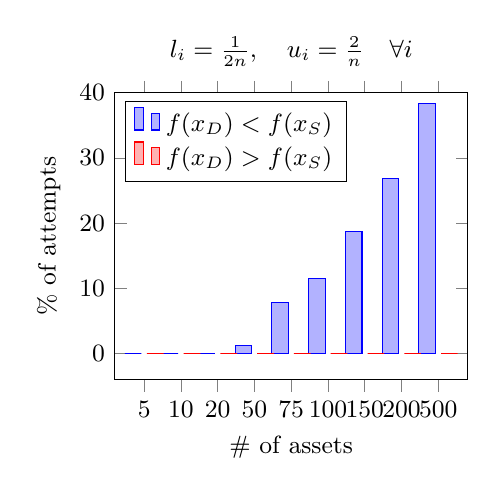
\begin{tikzpicture}
\begin{axis}[%
ybar,
xlabel={\# of assets},
ylabel={\% of attempts},
ylabel near ticks,
legend pos=north west,
symbolic x coords = {5,10,20,50,75,100,150,200,500},
bar width=6pt,
xtick=data,
ymax=40,
width=.5\textwidth,
title={$l_i = \frac{1}{2n}, \quad u_i = \frac{2}{n} \quad \forall i$},
]
\addplot coordinates { 
(5,0)         
(10,0)
(20,0)
(50,1.2)
(75,7.8)
(100,11.5)
(150,18.7)
(200,26.9)
(500,38.4)
 };
 
 \addplot coordinates { 
(5,0)         
(10,0)
(20,0)
(50,0)
(75,0)
(100,0)
(150,0)
(200,0)
(500,0)
 };

\addlegendentry{$f(x_{D}) < f(x_{S})$}
\addlegendentry{$f(x_{D}) > f(x_{S})$}
\end{axis}
\end{tikzpicture}


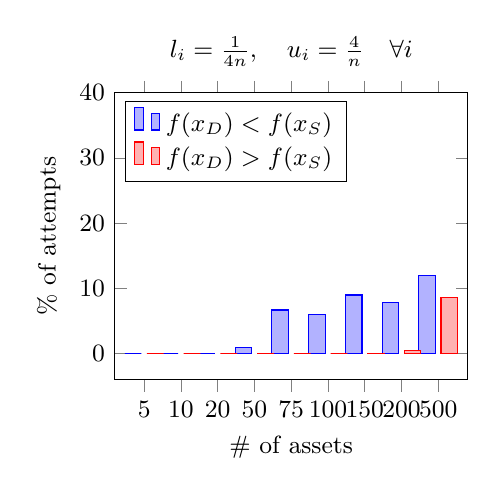
\begin{tikzpicture}
\begin{axis}[%
ybar,
xlabel={\# of assets},
ylabel={\% of attempts},
ylabel near ticks,
legend pos=north west,
symbolic x coords = {5,10,20,50,75,100,150,200,500},
bar width=6pt,
xtick=data,
ymax=40,
width=.5\textwidth,
title={$l_i = \frac{1}{4n}, \quad u_i = \frac{4}{n} \quad \forall i$}
]
\addplot coordinates { 
(5,0)         
(10,0)
(20,0)
(50,1.0)
(75,6.7)
(100,6.0)
(150,9.0)
(200,7.9)
(500,12.0)
 };
 
 \addplot coordinates { 
(5,0)         
(10,0)
(20,0)
(50,0)
(75,0)
(100,0)
(150,0.1)
(200,0.5)
(500,8.6)
 };

\addlegendentry{$f(x_{D}) < f(x_{S})$}
\addlegendentry{$f(x_{D}) > f(x_{S})$}
\end{axis}
\end{tikzpicture}
}

\makebox[\textwidth][c]{
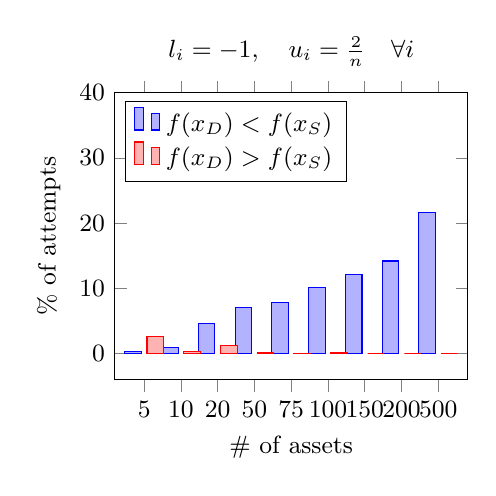
\begin{tikzpicture}
\begin{axis}[%
ybar,
xlabel={\# of assets},
ylabel={\% of attempts},
ylabel near ticks,
legend pos=north west,
symbolic x coords = {5,10,20,50,75,100,150,200,500},
bar width=6pt,
xtick=data,
ymax=40,
width=.5\textwidth,
title={$l_i = -1, \quad u_i = \frac{2}{n} \quad \forall i$}
]
\addplot coordinates { 
(5,0.3)         
(10,1.0)
(20,4.7)
(50,7.1)
(75,7.8)
(100,10.2)
(150,12.2)
(200,14.2)
(500,21.7)
 };
 
 \addplot coordinates { 
(5,2.7)         
(10,0.4)
(20,1.2)
(50,0.2)
(75,0.1)
(100,0.2)
(150,0)
(200,0)
(500,0)
 };

\addlegendentry{$f(x_{D}) < f(x_{S})$}
\addlegendentry{$f(x_{D}) > f(x_{S})$}
\end{axis}
\end{tikzpicture}
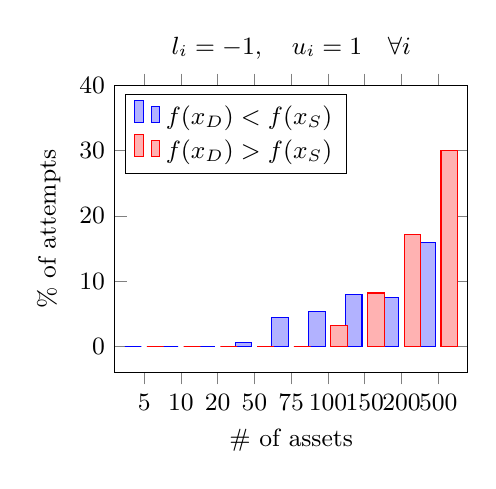
\begin{tikzpicture}
\begin{axis}[%
ybar,
xlabel={\# of assets},
ylabel={\% of attempts},
ylabel near ticks,
legend pos=north west,
symbolic x coords = {5,10,20,50,75,100,150,200,500},
bar width=6pt,
xtick=data,
ymax=40,
width=.5\textwidth,
title={$l_i = -1, \quad u_i = 1 \quad \forall i$}
]
\addplot coordinates { 
(5,0)         
(10,0)
(20,0)
(50,0.6)
(75,4.4)
(100,5.3)
(150,8.0)
(200,7.5)
(500,15.9)
 };
 
 \addplot coordinates { 
(5,0)         
(10,0)
(20,0)
(50,0)
(75,0)
(100,3.2)
(150,8.2)
(200,17.1)
(500,30)
 };

\addlegendentry{$f(x_{D}) < f(x_{S})$}
\addlegendentry{$f(x_{D}) > f(x_{S})$}
\end{axis}
\end{tikzpicture}
}
\caption{Comparison of objective function values for $x_{D}$ and $x_{S}$ with different box constraints. For each $n$ we perform $1000$ experiments for both the algorithms.}
\label{fig:box}
\end{figure}

In Figure (\ref{subfig-1:time1}) we compare the average execution time of the decomposition algorithm (with different values of $\lambda$) against SNOPT using 
\begin{equation}
x^0_i = \frac{1}{n} \quad \forall i
\end{equation}
and 
\begin{equation}\label{eq:generalbox}
l_i = \frac{1}{2n} \quad \forall i \qquad u_i = \frac{2}{n}  \quad \forall i
\end{equation} 
The $\epsilon$ in the stop criterion (\ref{eq:stop}) is set to $10^{-10}$. In Figure (\ref{subfig-2:iterations1}) we compare the average number of iterations performed by the decomposition algorithm using different values of $\lambda$.
\begin{figure}
\makebox[\textwidth][c]{
\subfloat[Comparison of average execution time\label{subfig-1:time1}]{
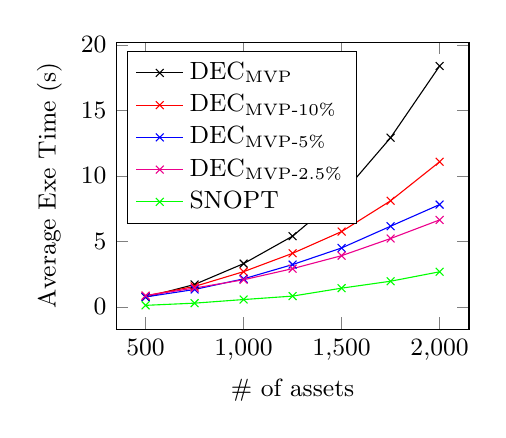
\begin{tikzpicture}
\begin{axis}[%
width=0.5\textwidth,
xlabel={\# of assets},
ylabel={Average Exe Time (s)},
scaled y ticks=false,
legend pos=north west,
legend cell align=left
]

\addplot [color=black,solid,mark=x,mark options={solid}]
  table[row sep=crcr]{%
%100	.105\\
%200	.214\\
%300	.340\\
500	.737	\\
750	1.713		\\
1000 3.303 \\
1250 5.400 \\
1500 8.56\\
1750 12.92\\
2000 18.39\\
};

\addplot [color=red,solid,mark=x,mark options={solid}]
  table[row sep=crcr]{%10
%100 .146\\
%250 .341\\
500 .853\\
750 1.56\\
1000 2.69 \\
1250 4.09\\
1500 5.75\\
1750 8.10\\
2000 11.08\\
};

\addplot [color=blue,solid,mark=x,mark options={solid}]
  table[row sep=crcr]{%5
%100 .190\\
%250 .355\\
500 .759 \\
750 1.33 \\
1000 2.14 \\
1250 3.23\\
1500 4.50 \\
1750 6.16 \\
2000 7.81 \\
};

\addplot [color=magenta,solid,mark=x,mark options={solid}]
  table[row sep=crcr]{%2.5
%100 .299\\
%250 .468\\
500  .854\\
750  1.44\\
1000 2.07 \\
1250 2.92 \\
1500 3.91 \\
1750 5.22 \\
2000 6.64\\
};
\addplot [color=green,solid,mark=x,mark options={solid}]
  table[row sep=crcr]{%
%100	.005	\\
%200	.014	\\
%300	.035	    \\
500	.118	    \\
750	 .286  \\
1000 0.561	\\
1250 0.824	\\
1500 1.43 \\
1750 1.96 \\
2000 2.68\\
};

\addlegendentry{DEC$_{\text{MVP}}$}
\addlegendentry{DEC$_{\text{MVP-}10\%}$}
\addlegendentry{DEC$_{\text{MVP-}5\%}$}
\addlegendentry{DEC$_{\text{MVP-}2.5\%}$}
\addlegendentry{SNOPT}
\end{axis}

\end{tikzpicture}
}
\hfill
\hspace{1em}\subfloat[Comparison of average iterations\label{subfig-2:iterations1}]{%
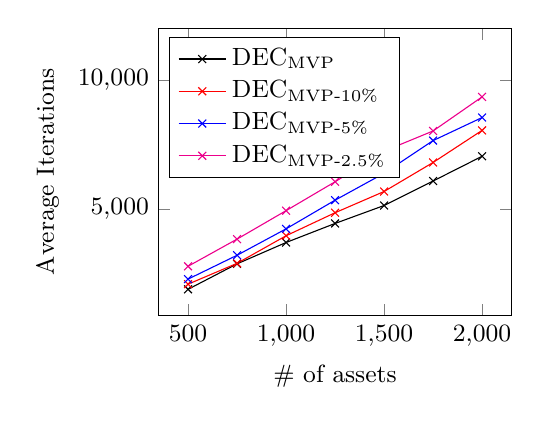
\begin{tikzpicture}

\begin{axis}[%
width=0.5\textwidth,
xlabel={\# of assets},
ylabel={Average Iterations},
ymax=12000,
scaled y ticks=false,
legend pos=north west,
legend cell align=left
]

\addplot [color=black,solid,mark=x,mark options={solid}]
  table[row sep=crcr]{%MVP
%100	445 \\
%200	819 \\
%300	1176 \\
500	1888\\
750	2874 \\
1000	 3701\\
1250	 4439\\
1500 5134\\
1750 6082\\
2000 7041\\
};

\addplot [color=red,solid,mark=x,mark options={solid}]
  table[row sep=crcr]{%10
%100 607\\
%250 1134\\
500 2087\\ 
750 2895 \\
1000 3962 \\
1250 4854 \\
1500 5676 \\
1750 6800 \\
2000 8043\\
};

\addplot [color=blue,solid,mark=x,mark options={solid}]
  table[row sep=crcr]{%5
%100 841\\
%250 1349\\
500 2283   \\
750 3207 \\
1000 4229  \\
1250 5340 \\
1500 6382 \\
1750 7648\\
2000 8541\\
};

\addplot [color=magenta,solid,mark=x,mark options={solid}]
  table[row sep=crcr]{%2.5
%100 1346\\
%250 1857\\
500 2780 \\
750 3832\\
1000 4934  \\
1250 6053\\
1500 7238\\
1750 8021\\
2000 9341\\
};

\addlegendentry{DEC$_{\text{MVP}}$}
\addlegendentry{DEC$_{\text{MVP-}10\%}$}
\addlegendentry{DEC$_{\text{MVP-}5\%}$}
\addlegendentry{DEC$_{\text{MVP-}2.5\%}$}
\end{axis}

\end{tikzpicture}
}
}
\caption{Comparison of performances using $\epsilon = 10^{-10}$ in (\ref{eq:stop}) with box constraints defined in (\ref{eq:generalbox})}
\end{figure}

\subsubsection{Classical box constraints}
In this section we use 
\begin{equation}\label{eq:classicalbox}
l_i = 0 \quad \forall i \qquad u_i = 1  \quad \forall i
\end{equation} 
In Figure (\ref{fig:100}) and Figure (\ref{fig:10}) we compare the average execution time and the average number of iterations performed by the decomposition algorithm (with different values of $\lambda$) against SNOPT using 
\begin{equation}
x^0 = \left[1, 0, .., 0 \right]
\end{equation}
The $\epsilon$ in the stop criterion (\ref{eq:stop}) is set to $10^{-10}$. In Figure (\ref{fig:100}) we set $M=100$, while in Figure (\ref{fig:10}) we set $M=10$.
\begin{figure}
\makebox[\textwidth][c]{
\subfloat[Comparison of average execution time\label{subfig-1:time2}]{%
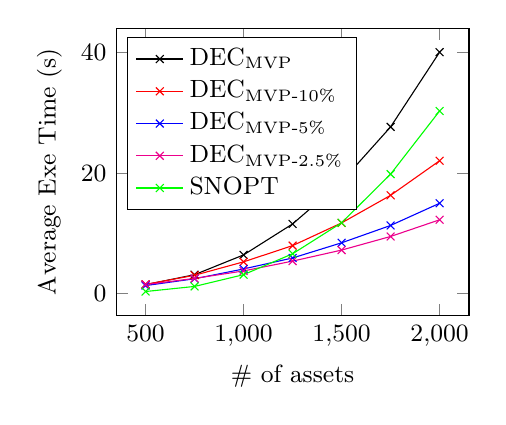
\begin{tikzpicture}
\begin{axis}[%
width=0.5\textwidth,
xlabel={\# of assets},
ylabel={Average Exe Time (s)},
scaled y ticks=false,
legend pos=north west,
legend cell align=left
]

\addplot [color=black,solid,mark=x,mark options={solid}]
  table[row sep=crcr]{%MVP
500	1.486	\\
750	3.147	\\
1000 6.431 \\
1250 11.57 \\
1500 18.6  \\
1750 27.68 \\
2000 40.08\\
};

\addplot [color=red,solid,mark=x,mark options={solid}]
  table[row sep=crcr]{%10
500 1.54\\
750 3.05\\
1000 5.28 \\
1250 7.97\\
1500 11.74\\
1750 16.32\\
2000 22.06\\
};

\addplot [color=blue,solid,mark=x,mark options={solid}]
  table[row sep=crcr]{%5
500 1.34 \\
750 2.47 \\
1000 4.10 \\
1250 5.92\\
1500 8.44 \\
1750 11.32 \\
2000 15.00 \\
};

\addplot [color=magenta,solid,mark=x,mark options={solid}]
  table[row sep=crcr]{%2.5
500  1.50\\
750  2.53\\
1000 3.77 \\
1250 5.40 \\
1500 7.23 \\
1750 9.49 \\
2000 12.26\\
};

\addplot [color=green,solid,mark=x,mark options={solid}]
  table[row sep=crcr]$}
\addlegendentry{DEC$_{\text{MVP-}5\%}$}
\addlegendentry{DEC$_{\text{MVP-}2.5\%}$}
\addlegendentry{SNOPT}
\end{axis}

\end{tikzpicture}
}
\hfill
\hspace{1em}\subfloat[Comparison of average iterations\label{subfig-2:iterations2}]{%
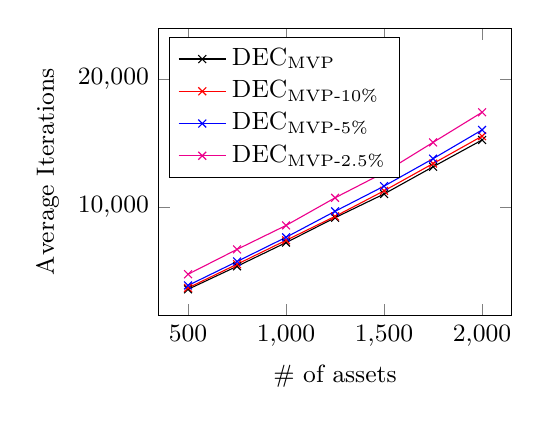
\begin{tikzpicture}

\begin{axis}[%
width=0.5\textwidth,
xlabel={\# of assets},
ylabel={Average Iterations},
scaled y ticks=false,
ymax=24000,
legend pos=north west,
legend cell align=left
]

\addplot [color=black,solid,mark=x,mark options={solid}]
  table[row sep=crcr]{%MVP
500	 3538\\
750	 5343 \\
1000	  7200\\
1250 	9151\\
1500    11011\\
1750 13141\\
2000 15241\\
};

\addplot [color=red,solid,mark=x,mark options={solid}]
  table[row sep=crcr]{%10
500 3644  \\
750 5503 \\
1000 7377 \\
1250 9255 \\
1500 11257 \\
1750 13392 \\
2000 15540\\
};

\addplot [color=blue,solid,mark=x,mark options={solid}]
  table[row sep=crcr]{%5
500 3840   \\
750 5719 \\
1000 7616  \\
1250 9652 \\
1500 11624 \\
1750 13776\\
2000 16029 \\
};

\addplot [color=magenta,solid,mark=x,mark options={solid}]
  table[row sep=crcr]$}
\addlegendentry{DEC$_{\text{MVP-}5\%}$}
\addlegendentry{DEC$_{\text{MVP-}2.5\%}$}
\end{axis}

\end{tikzpicture}
}
}
\caption{Comparison of performances using $\epsilon = 10^{-10}$ in (\ref{eq:stop}) with box constraints defined in (\ref{eq:classicalbox}) with $M=100$}
\label{fig:100}
\end{figure}

\begin{figure}
\centering
\makebox[\textwidth][c]{
\subfloat[Comparison of average execution time\label{subfig-1:time3}]{%
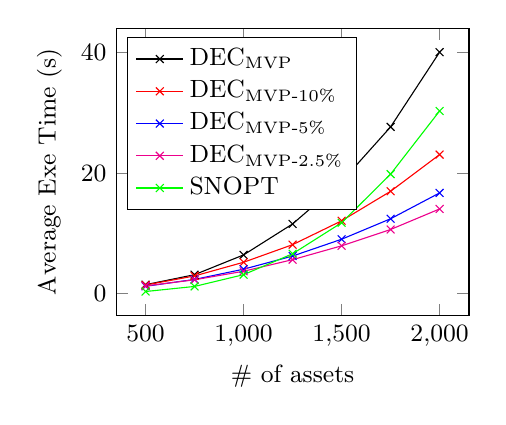
\begin{tikzpicture}
\begin{axis}[%
width=0.5\textwidth,
xlabel={\# of assets},
ylabel={Average Exe Time (s)},
scaled y ticks=false,
legend pos=north west,
legend cell align=left
]

\addplot [color=black,solid,mark=x,mark options={solid}]
  table[row sep=crcr]{%MVP
500	1.486	\\
750	3.147	\\
1000 6.431 \\
1250 11.57 \\
1500 18.6  \\
1750 27.68 \\
2000 40.08\\
};

\addplot [color=red,solid,mark=x,mark options={solid}]
  table[row sep=crcr]{%10
500 1.43\\
750 2.94\\
1000 5.21 \\
1250 8.13\\
1500 12.09\\
1750 16.99\\
2000 23.08\\
};

\addplot [color=blue,solid,mark=x,mark options={solid}]
  table[row sep=crcr]{%5
500 1.22 \\
750 2.36 \\
1000 4.06 \\
1250 6.24\\
1500 9.03 \\
1750 12.43 \\
2000 16.72 \\
};

\addplot [color=magenta,solid,mark=x,mark options={solid}]
  table[row sep=crcr]{%2.5
500  1.28\\
750  2.30\\
1000 3.72 \\
1250 5.64 \\
1500 7.94 \\
1750 10.65 \\
2000 14.06\\
};

\addplot [color=green,solid,mark=x,mark options={solid}]
  table[row sep=crcr]$}
\addlegendentry{DEC$_{\text{MVP-}5\%}$}
\addlegendentry{DEC$_{\text{MVP-}2.5\%}$}
\addlegendentry{SNOPT}
\end{axis}

\end{tikzpicture}
}
\hfill
\hspace{1em}\subfloat[Comparison of average iterations\label{subfig-2:iterations3}]{%
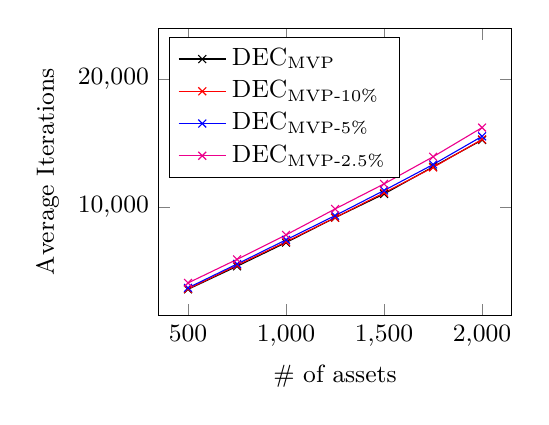
\begin{tikzpicture}

\begin{axis}[%
width=0.5\textwidth,
xlabel={\# of assets},
ylabel={Average Iterations},
scaled y ticks=false,
legend pos=north west,
legend cell align=left,
ymax=24000
]

\addplot [color=black,solid,mark=x,mark options={solid}]
  table[row sep=crcr]{%MVP
500	 3538\\
750	 5343 \\
1000	  7200\\
1250 	9151\\
1500    11011\\
1750 13141\\
2000 15241\\
};

\addplot [color=red,solid,mark=x,mark options={solid}]
  table[row sep=crcr]{%10
500 3565  \\
750 5422 \\
1000 7263 \\
1250 9155 \\
1500 11101 \\
1750 13089 \\
2000 15289\\
};

\addplot [color=blue,solid,mark=x,mark options={solid}]
  table[row sep=crcr]{%5
500 3654   \\
750 5522 \\
1000 7418  \\
1250 9314 \\
1500 11285 \\
1750 13317\\
2000 15526\\
};

\addplot [color=magenta,solid,mark=x,mark options={solid}]
  table[row sep=crcr]$}
\addlegendentry{DEC$_{\text{MVP-}5\%}$}
\addlegendentry{DEC$_{\text{MVP-}2.5\%}$}
\end{axis}

\end{tikzpicture}
}
}
\caption{Comparison of performances using $\epsilon = 10^{-10}$ in (\ref{eq:stop}) with box constraints defined in (\ref{eq:classicalbox}) with $M=10$}
\label{fig:10}
\end{figure}

\subsubsection{Convergence to a Risk Parity solution}
In this section we evaluate the probability to converge to a critical point $(x^*,y^*)$ that is also a Risk Parity solution, i.e. that satisfies 
\begin{equation}\label{eq:reseps}
\max_i \left| \frac{RC_i}{\mathcal{R}(x^*,y^*)} - \frac{1}{n} \right| < 10^{-6}
\end{equation}
where $RC_i$ is the risk contribution of the asset $i$ and ${\mathcal{R}(x^*,y^*)}$ is the total risk of the invested portfolio. Equation (\ref{eq:reseps}) express the fact that the (normalized) max deviation from Risk Parity of the solutions is less than $10^{-6}$. In Figure (\ref{fig:convergence1}) we compare the probability to reach a Risk Parity solution for both the decomposition algorithm (with different values of $\lambda$) and SNOPT. 

\begin{figure}
\makebox[\textwidth][c]{
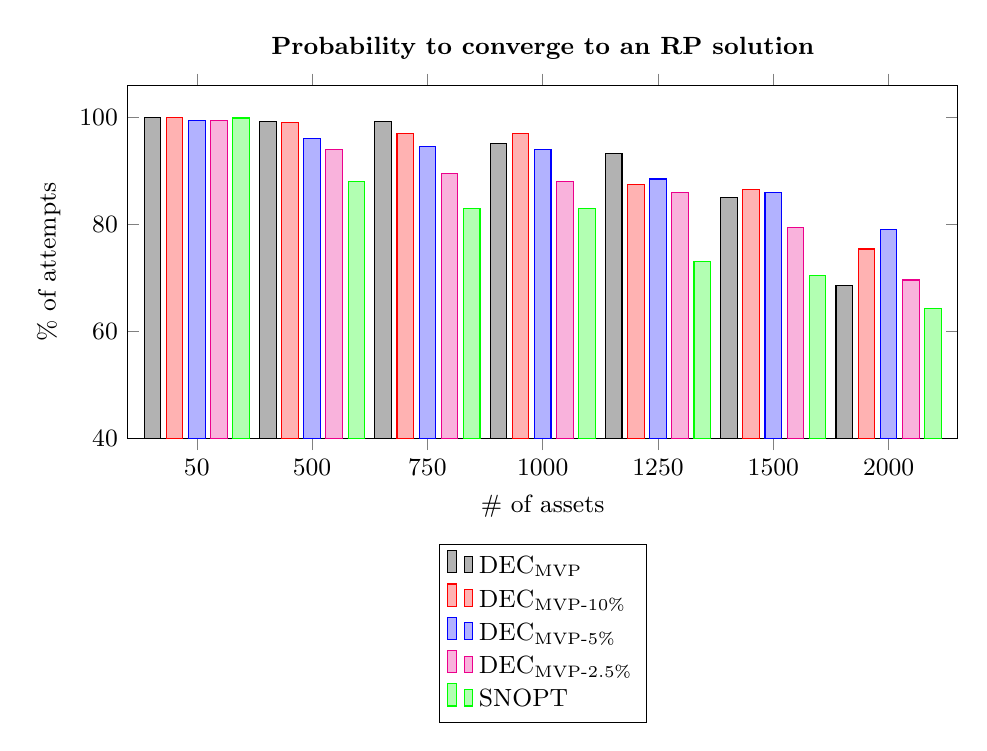
\begin{tikzpicture}
\begin{axis}[%
ybar,
width=1\textwidth,
height=0.5\textwidth,
xlabel={\# of assets},
ylabel={\% of attempts},
ylabel near ticks,
legend pos=south west,
symbolic x coords = {5, 50, 500, 750, 1000, 1250, 1500, 2000},
bar width=6pt,
xtick=data,
ymin=40,
title=\textbf{Probability to converge to an RP solution},
legend cell align=left,
legend style={at={(0.5,-0.3)},anchor=north}
]

 
 \addplot [color=black ,fill=black, fill opacity=0.3] coordinates { %MVP
%(5,100)
(50,100)
(500,99.2)
(750,99.2)
(1000,95.2)
(1250,93.2)
(1500,85.0)
(2000,68.5)
 };
 
\addplot [color=red,fill=red, fill opacity=0.3] coordinates { % 10%
%(5,100)
(50,100)
(500,99.0)     
(750,97.0)    
(1000,97.0)
(1250,87.5)
(1500,86.5)
(2000,75.4)
 };
 
 \addplot [color=blue, fill=blue, fill opacity=0.3] coordinates { % 5%
%(5,100)   
(50,99.5)
(500,96.0)
(750,94.5)
(1000,94)
(1250,88.5)
(1500,86)
(2000,79)
 };
 
 \addplot [color=magenta, fill=magenta, fill opacity=0.3] coordinates { % 2.5%
%(5,100)   
(50,99.5)
(500,94)
(750,89.5)
(1000,88)
(1250,86)
(1500,79.5)
(2000,69.6)
 }; 
 
\addplot [color=green, fill=green, fill opacity=0.3] coordinates { 
%(5,100)         
(50,99.9)
(500,88)
(750,83)
(1000,83)
(1250,73)
(1500,70.5)
(2000,64.2)
 };


\addlegendentry{DEC$_{\text{MVP}}$}
\addlegendentry{DEC$_{\text{MVP-}10\%}$}
\addlegendentry{DEC$_{\text{MVP-}5\%}$}
\addlegendentry{DEC$_{\text{MVP-}2.5\%}$}
\addlegendentry{SNOPT}
\end{axis}
\end{tikzpicture}
}
\caption{Probability to converge to a Risk Parity solution using $x^{0}= [1, 0, .., 0]$ for the decomposition algorithm (with different values of $\lambda$) and SNOPT.}
\label{fig:convergence1}
\end{figure}

%\begin{table}
%\centering
%\begin{tabular}{ c | c | c | c }
%n &  G-S$_{(ALS)}$ & G-S$_{(ELS)}$  & SNOPT \\\hline
%5    & 100.0\% & 100.0\% & 100.0\%\\\hline
%10   & 100.0\% & 100.0\% & 100.0\%\\\hline
%20   & 100.0\% & 100.0\% & 100.0\%\\\hline
%50   & 99.0\%  & 99.4\%  & 99.5\%\\\hline
%100  & 85.4\%  & 87.0\%  & 91.2\%\\\hline
%200  & 40.0\%  & 45.0\%  & 52.0\%\\\hline
%300  & 22.0\%  & 24.0\%  & 34.0\%\\\hline
%500  & 0.0\%   & 6.0\%   & 3.0\%\\\hline
%750  & 0.0\%   & 2.0\%   & 0.0\%\\\hline
%1000 & 0.0\%   & 0.0\%   & 0.0\%\\\hline
%1250 & 0.0\%   & 0.0\%   & 0.0\%\\\hline
%\end{tabular}
%\caption{Probability to converge to a Risk Parity solution using $x^{0}_i = 1/n \quad \forall i$}
%\label{tab:first}
%\end{table}
%
%
%\begin{table}
%\centering
%\begin{tabular}{ c | c | c | c}
%n &  G-S$_{(ALS)}$ & G-S$_{(ELS)}$  & SNOPT \\\hline
%5    & 100.0\%  & 100.0\% & 100.0\%\\\hline
%10   & 100.0\%  & 100.0\% & 99.9\%\\\hline
%20   & 100.0\%  & 100.0\%  & 100.0\%\\\hline
%50   & 100.0\%  & 99.9\%  & 99.9\%\\\hline
%100  & 99.9\%   & 100.0\%  & 99.6\% \\\hline
%200  & 100.0\%  & 100.0\%  & 98.8\% \\\hline
%300  & 100.0\%  & 100.0\%  & 96.6\% \\\hline
%500  & 99.5\%   & 99.2\%   & 88.0\%\\\hline
%750  & 99.5\%   & 99.2\%  & 83.0\%\\\hline
%1000 & 98.0\%   & 95.2\%  & 83.0\%\\\hline
%1250 & 91.5\%   & 93.2\%  & 73.0\%\\\hline
%\end{tabular}
%\caption{Probability to converge to a Risk Parity solution using $x^{0}= [1, 0, .., 0]$}
%\label{tab:second}
%\end{table}

\subsubsection{On the choosing of starting point}
From our experiments, it turns out that the choice of the starting point $x^0$ strongly affects the probability of the algorithms to reach a Risk Parity solution.  In Figure (\ref{fig:sparsity}) we measure the probability to reach a Risk Parity solution varying the sparsity of the initial guess $x^0$, i.e. the percentage of components of $x^0$ fixed to 0. In Figure (\ref{subfig-3:equally}) we use an equally distributed starting point:
\begin{equation}
x^{0} = \left[x^{0}_0, x^{0}_1, .. ,  x^{0}_k, x^{0}_{k+1} .., x^{0}_n \right] = \left[\frac{1}{k}, \frac{1}{k}, .., \frac{1}{k}, 0, .., 0 \right]
\end{equation}
In Figure (\ref{subfig-3:random}) we use a randomly distributed starting point:
\begin{equation}
\begin{aligned}
&a^{0} = \left[r_0, r_1, ..,r_k, 0, .., 0 \right] \qquad \text{where} \quad r_i \sim \mathcal{U}[0,1]\\
&x^0 = \frac{a^{0}}{\mathds{1}^T a^0}
\end{aligned}
\end{equation}

\begin{figure}
\makebox[\textwidth][c]{
\hspace{1em}\subfloat[With equally distributed $x_0$\label{subfig-3:equally}]{%
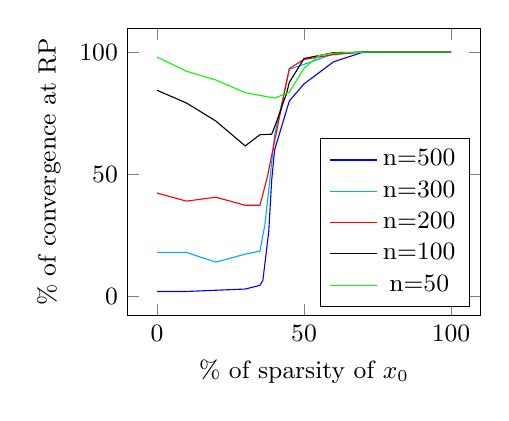
\begin{tikzpicture}
\begin{axis}[%
xlabel={\% of sparsity of $x_0$},
ylabel={\% of convergence at RP},
scaled y ticks=false,
width=0.5\textwidth,
legend pos=south east
]

\addplot [color=blue,solid,mark=none,mark options={solid}]
  table[row sep=crcr]{%
0 2 \\
10 2 \\
20 2.5 \\
30 3 \\
35 4.5 \\
36 6.5
37 14.5 \\
38 26.5 \\
39 47.5 \\
40 60 \\
45 80\\
50 87 \\
60 96 \\
70 100 \\
80 100 \\
90 100 \\
100 100 \\
};

\addplot [color=cyan,solid,mark=none,mark options={solid}]
  table[row sep=crcr]{%
0 18\\
10 18 \\
20 14 \\
30 17.3 \\
35 18.5 \\
36.67 29.1 \\
38.3 47 \\
40 66 \\
45 93 \\
50 95 \\
60 99.3 \\
70 100 \\
80 100 \\
90 100 \\
100 100\\
};

\addplot [color=red,solid,mark=none,mark options={solid}]
  table[row sep=crcr]{%
0 42.3 \\
10 39 \\
20 40.6 \\
30 37.3 \\
35 37.3 \\
37.5 48.7 \\
38.5 54.7 \\
40 63.6 \\
45 93.3 \\
50 97 \\
60 99 \\
70 100 \\
80 100 \\
90 100 \\
100 100\\
};

\addplot [color=black,solid,mark=none,mark options={solid}]
  table[row sep=crcr]{%
0 84.4 \\
10 79.2 \\
20 71.8 \\
30 61.6 \\
35 66.2 \\
39 66.4 \\
40 69.4 \\
42 76 \\
43 79.6 \\
44 82.8\\
45 87.6 \\
50 97.4 \\
60 99.8 \\
70 100 \\
80 100 \\
90 100 \\
100 100\\
};

\addplot [color=green,solid,mark=none,mark options={solid}]
  table[row sep=crcr]{%
0 98 \\
10 92.2 \\
20 88.6\\
30 83.4 \\
40 81.2 \\
45 83.6 \\
50 93.4 \\
55 98.6 \\
60 99.6 \\
70 100 \\
80 100 \\
90 100 \\
100 100 \\
};
\addlegendentry{n=500}
\addlegendentry{n=300}
\addlegendentry{n=200}
\addlegendentry{n=100}
\addlegendentry{n=50}
\end{axis}
\end{tikzpicture}
}
\hspace{1em}\subfloat[With random $x_0$\label{subfig-3:random}]{%
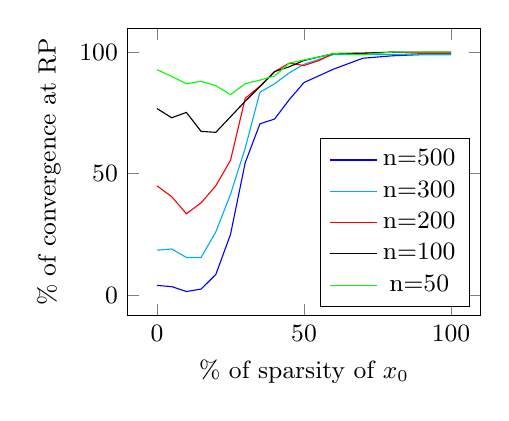
\begin{tikzpicture}
\begin{axis}[%
width=0.5\textwidth,
xlabel={\% of sparsity of $x_0$},
ylabel={\% of convergence at RP},
legend pos=south east
]

\addplot [color=blue,solid,mark=none,mark options={solid}]
  table[row sep=crcr]{%
0  4.0 \\
5  3.5 \\
10 1.5 \\
15 2.5 \\
20 8.5 \\
25 25.0 \\
30 54.5 \\
35 70.5 \\
40 72.5 \\
45 80.5 \\
50 87.5 \\
60 93 \\
70 97.5 \\
80 98.5 \\
90 99.0 \\
100 99.0 \\
};

\addplot [color=cyan,solid,mark=none,mark options={solid}]
  table[row sep=crcr]{%
0 18.5 \\
5 19.0 \\
10 15.5 \\
15 15.5 \\
20 26.0 \\
25 41.5 \\
30 60.5 \\
35 83.5 \\
40 87.0 \\
45 91.5 \\
50 95.0 \\
60 99.0 \\
90 99.0 \\
100 99.0 \\
};

\addplot [color=red,solid,mark=none,mark options={solid}]
  table[row sep=crcr]{%
0 45 \\
5 40.5 \\
10 33.5 \\
15 38.0 \\
20 45.0 \\
25 55.5 \\
30 81.0 \\
35 86.0 \\
40 92.0 \\
45 95.5 \\
50 94.5 \\
55 96.5 \\
60 99.5 \\
70 99.5 \\
80 100 \\
90 99.5 \\
100 99.5 \\
};

\addplot [color=black,solid,mark=none,mark options={solid}]
  table[row sep=crcr]{%
0 76.8 \\
5 73 \\
10 75.2 \\
15 67.4 \\
20 67 \\
25 73.4 \\
30 79.8 \\
35 85.8 \\
40 92 \\
45 94 \\
50 96.6 \\
55 98 \\
60 99.4 \\
70 99.6 \\
80 100 \\
90 100 \\
100 100 \\
};

\addplot [color=green,solid,mark=none,mark options={solid}]
  table[row sep=crcr]{%
0 92.8\\
5 90 \\
10 87.0 \\
15 88.0 \\
20 86.2\\
25 82.5 \\
30 87.0 \\
35 88.5 \\
40 90.2 \\
45 95.5 \\
50 96.8 \\
55 98.0 \\
60 99.4 \\
70 99.0 \\
80 100 \\
90 100 \\
100 100\\
};


\addlegendentry{n=500}
\addlegendentry{n=300}
\addlegendentry{n=200}
\addlegendentry{n=100}
\addlegendentry{n=50}
\end{axis}
\end{tikzpicture}
}
}
\caption{Percentage of computations of DEC$_{\text{MVP}}$ that find an RP solution, varying the sparsity of the initial guess $x^0$, for different number of assets $n$}
\label{fig:sparsity}
\end{figure}



\clearpage
%% The Appendices part is started with the command \appendix;
%% appendix sections are then done as normal sections
%% \appendix

%% \section{}
%% \label{}

%% If you have bibdatabase file and want bibtex to generate the
%% bibitems, please use
%%
%%  \bibliographystyle{elsarticle-num} 
%%  \bibliography{<your bibdatabase>}

%% else use the following coding to input the bibitems directly in the
%% TeX file.

\begin{thebibliography}{00}
\section{Bibliography}
\bibitem{maillard}
S. Maillard, T. Roncalli, J. Teiletche,
\emph{On the properties of equally weighted risk contribution portfolios}, 
2010.

\bibitem{tutuncu}
  X. Bai, K. Scheinberg, R. Tutuncu,
  \emph{Least-square approach to risk parity in portfolio selection},
  2013.   
  
\bibitem{snopt}
	P. E. Gill, W. Murray, M. A. Sanders,
	\emph{SNOPT: An SQP Algorithm for large-scale constrained optimization}, 
	2005.


\end{thebibliography}
\end{document}
\endinput
%%
%% End of file `elsarticle-template-num.tex'.
